\usepackage{listings}%! suppress = LineBreak
%%
%% This is file `sample-sigconf.tex',
%% generated with the docstrip utility.
%%
%% The original source files were:
%%
%% samples.dtx  (with options: `sigconf')
%%
%% IMPORTANT NOTICE:
%%
%% For the copyright see the source file.
%%
%% Any modified versions of this file must be renamed
%% with new filenames distinct from sample-sigconf.tex.
%%
%% For distribution of the original source see the terms
%% for copying and modification in the file samples.dtx.
%%
%% This generated file may be distributed as long as the
%% original source files, as listed above, are part of the
%% same distribution. (The sources need not necessarily be
%% in the same archive or directory.)
%%
%% The first command in your LaTeX source must be the \documentclass command.
\documentclass[sigconf,review,anonymous]{acmart}


% Packages
\usepackage{amsfonts}
\usepackage{amsmath}
\usepackage{graphicx}
\usepackage{hyperref}
\usepackage{float}
\usepackage{pgfplots}
\usepgfplotslibrary{fillbetween}
\usepackage[pdf]{graphviz}
\usepackage{tikz}
\usepackage{natbib}

\usepackage{booktabs}
\usepackage{pifont}
\usepackage{fontspec}
\usepackage{fontawesome}

\newcommand{\wmark}{\textcolor{orange}{\ding{45}}}
\newcommand{\cmark}{\textcolor{green!80!black}{\ding{51}}}
\newcommand{\xmark}{\textcolor{red}{\ding{55}}}

\usepackage{multicol}

% Packages
\usepackage{amsmath}
\usepackage{listings}
\usepackage{fontspec}
\usepackage{xcolor}

\setmonofont{JetBrainsMono}[
  Contextuals={Alternate},
  Path=./JetbrainsFontFiles/,
  Extension = .ttf,
  UprightFont=*-Regular,
  BoldFont=*-Bold,
  ItalicFont=*-Italic,
  BoldItalicFont=*-BoldItalic
]

\makeatletter
\def\verbatim@nolig@list{}
\makeatother

\lstdefinelanguage{kotlin}{
  comment=[l]{//},
  commentstyle={\color{gray}\ttfamily},
  emph={delegate, filter, firstOrNull, forEach, it, lazy, mapNotNull, println, repeat, assert, with, head, tail, len, return@},
  numberstyle=\noncopyable,
  emphstyle={\color{OrangeRed}},
  identifierstyle=\color{black},
  keywords={abstract, actual, as, as?, break, by, class, companion, continue, data, do, dynamic, else, enum, expect, false, final, for, fun, get, if, import, in, infix, interface, internal, is, null, object, open, operator, override, package, private, public, return, sealed, set, super, suspend, this, throw, true, try, catch, typealias, val, var, vararg, when, where, while, tailrec, reified},
  keywordstyle={\color{NavyBlue}\bfseries},
  morecomment=[s]{/*}{*/},
  morestring=[b]",
  morestring=[s]{"""*}{*"""},
  ndkeywords={@Deprecated, @JvmField, @JvmName, @JvmOverloads, @JvmStatic, @JvmSynthetic, Array, Byte, Double, Float, Boolean, Int, Integer, Iterable, Long, Runnable, Short, String},
  ndkeywordstyle={\color{BurntOrange}\bfseries},
  sensitive=true,
  stringstyle={\color{ForestGreen}\ttfamily},
  literate={`}{{\char0}}1
}

\lstset{basicstyle=\ttfamily\lst@ifdisplaystyle\small\fi}

%% NOTE that a single column version may be required for
%% submission and peer review. This can be done by changing
%% the \doucmentclass[...]{acmart} in this template to
%% \documentclass[manuscript,screen]{acmart}
%%
%% To ensure 100% compatibility, please check the white list of
%% approved LaTeX packages to be used with the Master Article Template at
%% https://www.acm.org/publications/taps/whitelist-of-latex-packages
%% before creating your document. The white list page provides
%% information on how to submit additional LaTeX packages for
%% review and adoption.
%% Fonts used in the template cannot be substituted; margin
%% adjustments are not allowed.
%%
%%
%% \BibTeX command to typeset BibTeX logo in the docs
\AtBeginDocument{%
  \providecommand\BibTeX{{%
    \normalfont B\kern-0.5em{\scshape i\kern-0.25em b}\kern-0.8em\TeX}}}

%% Rights management information.  This information is sent to you
%% when you complete the rights form.  These commands have SAMPLE
%% values in them; it is your responsibility as an author to replace
%% the commands and values with those provided to you when you
%% complete the rights form.
\setcopyright{acmcopyright}
\copyrightyear{2022}
\acmYear{2022}
\acmDOI{10.1145/1122445.1122456}

%% These commands are for a PROCEEDINGS abstract or paper.


\acmConference[ICSE 2022]{The 44th International Conference on Software Engineering}{May 21–29, 2022}{Pittsburgh, PA, USA}


\newcommand{\seqWord}{Seq \langle Word \rangle}
\newcommand{\distSeqWord}{Dist\langle \seqWord  \rangle}

%%
%% Submission ID.
%% Use this when submitting an article to a sponsored event. You'll
%% receive a unique submission ID from the organizers
%% of the event, and this ID should be used as the parameter to this command.
%%\acmSubmissionID{123-A56-BU3}

%%
%% The majority of ACM publications use numbered citations and
%% references.  The command \citestyle{authoryear} switches to the
%% "author year" style.
%%
%% If you are preparing content for an event
%% sponsored by ACM SIGGRAPH, you must use the "author year" style of
%% citations and references.
%% Uncommenting
%% the next command will enable that style.
%%\citestyle{acmauthoryear}

%%
%% end of the preamble, start of the body of the document source.
\begin{document}

%%
%% The "title" command has an optional parameter,
%% allowing the author to define a "short title" to be used in page headers.
  \title{How robust is neural code completion to cosmetic variance?}
% \title{Code Transformations
% Neural language models
% Interpretability
% Reliability/Robustness
% Comprehension/Understanding

% }

% \title{An empirical study of source code transformations on the robustness of neural language models}
%%
%% The "author" command and its associated commands are used to define
%% the authors and their affiliations.
%% Of note is the shared affiliation of the first two authors, and the
%% "authornote" and "authornotemark" commands
%% used to denote shared contribution to the research.
  \author{Breandan Considine, Xujie Si, Jin L.C. Guo}
  \email{breandan.considine@mail.mcgill.ca, {xsi, jguo}@cs.mcgill.ca}
  \affiliation{%
    \institution{McGill University}
  }

%%
%% By default, the full list of authors will be used in the page
%% headers. Often, this list is too long, and will overlap
%% other information printed in the page headers. This command allows
%% the author to define a more concise list
%% of authors' names for this purpose.
% \renewcommand{\shortauthors}{Trovato and Tobin, et al.}

%%
%% The abstract is a short summary of the work to be presented in the
%% article.
  \begin{abstract}
    Neural language models hold great promise as tools for computer-aided programming, but questions remain over their reliability and the consequences of overreliance. In the domain of natural language, prior work has revealed these models can be sensitive to naturally-occurring variance and malfunction in unpredictable ways. A closer examination of neural language models is needed to understand their behavior in programming-related tasks. In this work, we develop a methodology for systematically evaluating neural code completion models using common source code transformations such as synonymous renaming, intermediate logging, and independent statement reordering. Applying these synthetic transformations to a dataset of handwritten code snippets, we evaluate three SoTA models, CodeBERT, GraphCodeBERT and RobertA-Java, which exhibit varying degrees of robustness to cosmetic variance. Our approach is implemented and released as a modular and extensible toolkit for evaluating code-based neural language models.


    % What is the key message?
    %   - Different types of SCTs
    %.  - Different types of deep learning models (e.g. RNNs, transformers)
    %   - Different types of Evaluation tasks (e.g. code completion)
    %.  - Different measures of robustness (e.g. latent space, predictions)
    %
  \end{abstract}

  \maketitle

  \section{Introduction}\label{sec:introduction}

  Neural language models play an increasingly synergetic role in software engineering, and are featured prominently in recent work on neural code completion~\cite{chen2021evaluating}. Yet from a development perspective, the behavior of these models is opaque: partially completed source code written inside an editor is sent to a remote server, which returns a completion. This client-server architecture can be seen as a black-box or \textit{extensional} function. How can we evaluate the behavior of neural language models in this setting? The value of automated testing becomes evident.

  First conceived in the software testing literature, metamorphic testing~\cite{chen1995metamorphic} is a concept known in machine learning as \textit{self-supervision}. In settings where labels are scarce but invariant to certain groups of transformation or \textit{metamorphic relations}, given a finite labeled dataset, one can generate an effectively infinite amount of synthetic data by selecting and recombining those transformations. For example, computer vision models should be invariant to shift, scale and rotation: given a small dataset of labeled images, we can apply these transformations to generate much larger training or validation set. Could similar invariants exist for source code?

  In this work, we aim to understand how well neural code completion models generalize to plausible perturbations. Do language models learn to recognize certain patterns or \textit{idioms} and if so, what kinds? A great deal of research has been undertaken~\citep{weiss2018practical, chirkova2020empirical, chen2021evaluating} to characterize the families of computational languages neural language models can recognize in practice. Our work builds on this literature from an engineering standpoint: we explore the extent to which neural code completion models are affected by cosmetic variation, by measuring the effect of various code transformations on three separate pretrained models. We compare the robustness of these models on two downstream tasks: code and document completion. Each model is evaluated on a set of synthetically altered code snippets, and predicts one or more masked tokens.

  Together, these transformations represent "possible worlds" in the tradition modal logic: the original author plausibly ``could have'' chosen such a way to express their ideas. Although we cannot access all these worlds, we can posit their existence and likelihood, given a large enough dataset of sufficiently similar code.

  Source code in semantically or even syntactically-equivalent programs has many degrees of freedom: two authors implementing the same function may select different variable names or cosmetic features, such as whitespaces, diagnostic statements or comments. One would expect neural code completion for languages semantically invariant under those changes to exhibit the same invariance: \textit{cosmetically-altered code snippets should not drastically change the model's predictions}. For example, code completion in Java should be invariant to variable renaming, whitespace placement, extra documentation or reordering dataflow-independent statements.

  One can make this statement slightly more formal. Given a neural code completion model \lstinline|ncc: Str->Str|, a list of code snippets, \lstinline|snps: List<Str>|, a masking procedure, \lstinline|msk: Str->Str|, a single cosmetic transformation, \lstinline|ctx: Str->Str|, and a code completion metric, \lstinline|mtr: (Str, Str)->Float|, we would expect the average completion accuracy to remain roughly unchanged regardless of whether the transformation was applied, i.e.,

  \noindent\begin{lstlisting}[basicstyle=\footnotesize\ttfamily, language=kotlin,label={lst:lstlisting}]
fun ctxVariance(ncc, snps, msk, ctx, mtr) = Δ(
  zip(snps, snps | msk | ncc) | mtr | average,
  zip(snps | ctx, snps | ctx | msk | ncc) | mtr | average
)
  \end{lstlisting}

  \noindent where \texttt{|} maps a function over a sequence, and \lstinline|zip| zips two sequences into a sequence of pairs. We assume \lstinline|snps| and \lstinline|msk| are fixed, and evaluate three different neural code completion models, five different transformations and two different metrics.


  \pagebreak\section{Method}

  Given a set of source code snippets of varying complexity, a set of SCTs, and a set of tasks, how do these factors affect model completion accuracy? To measure this, we first sample the top 100 most-starred Java repositories published by GitHub organizations with over 100 forks and between 1 and 10 MB in size. This ensures a diverse dataset of active repositories with a reasonable amount of quality and stylistic diversity. From these, we extract a set of Java methods using the heuristic described in \S\ref{sec:slicing}.

  Our goal then, is to measure the language models' robustness under various cosmetic changes. To do so, we generate and measure variance on various SCTs. To generate these SCTs, we implement a tool which generates synthetic variants of naturally-occurring source code snippets from each of the following categories and evaluates the model for completion accuracy. We have implemented the following source code transformations (SCTs):

  \begin{enumerate}
    \item \textbf{Synonym renaming}: rename variables with synonyms
    \item \textbf{Peripheral code}: introduce dead code to source code
    \item \textbf{Statement reordering}: swap independent statement order
    \item \textbf{Document generation}: add synthetic documentation
    \item \textbf{Permute argument order}: scramble method arguments
  \end{enumerate}

  Ideally, these would be generated using a higher-order abstract syntax to ensure syntactic validity, however for the sake of simplicity, we implemented the transformations using a set of ad-hoc regular expressions. While slightly awkward for implementing more complex transformations, we observed in practice this approach can effectively make cosmetic changes like variable renaming and linear statement reordering without much difficulty.

  For each SCT, we mask various tokens in the code snippet and compare the model's ability to fill in the correct token before and after the transformation is applied. Our goal is to measure how sensitive the pretrained model is to each type of SCT.

  \begin{figure}[H]
    \centering
    \includegraphics[width=0.35\textwidth]{figs/dataflow.png}
    \caption{For each code snippet, we apply a SCT and measure the model's shift in accuracy on some task, e.g. source code or document completion.}
    \label{fig:dataflow}
  \end{figure}

  Our framework encompasses both code completion and document synthesis. For example, we can treat code completion as a masked-token completion task, in which we sample several tokens from the original source code and the variant, then measure the average shift in model accuracy across the masked locations. This can be done either inside the model's latent space using a sensitivity margin, or using some metric on the output string. We decided to focus on the output space and consider two metrics: ROUGE-synonym and average multimask accuracy using top-1 softmax output. Consider the multimask completion task for a single snippet:

  \begin{lstlisting}[basicstyle=\scriptsize\ttfamily, language=kotlin,label={lst:example1}]
/**
 * Write to output buffer and compact
 */
public void write(int b) throws IOException {
  if (!buffer.hasRemaining()) {
    throw new IOException("OutputStream buffer is full");
  }
  buffer.put((byte) b);
  buffer.flip();
  sink();
  buffer.compact();
}
  \end{lstlisting}

  We sample k tokens and individually mask them separately, then have the model predict the masked token:

  \begin{lstlisting}[basicstyle=\scriptsize\ttfamily, language=kotlin,label={lst:example2}]
/**
 * Write to output buffer and compact
 */
public void <MASK>(int b) throws IOException {
  if (!buffer.hasRemaining()) {
    throw new IOException("OutputStream buffer is full");
  }
  buffer.<MASK>((byte) b);
  buffer.flip();
  sink();
  <MASK>.compact();
}
  \end{lstlisting}

  For each mask location, we collect model's completions, then for each SCT, measure the average distributional shift before and after applying the transformation.

  Similarly, for document synthesis, we discard the original comment in its entirety and sample tokens with greedy autoregressive decoding until a newline stopword is encountered. Here is a Javadoc generated by our document synthesizer using GraphCodeBERT:

  \begin{lstlisting}[basicstyle=\scriptsize\ttfamily, language=kotlin,label={lst:example3}]
/**
 * Write a single byte to the output stream.
 */
public void write(int b) throws IOException {
  if (!buffer.hasRemaining()) {
    throw new IOException("OutputStream buffer is full");
  }
  buffer.put((byte) b);
  buffer.flip();
  sink();
  buffer.compact();
}
  \end{lstlisting}

  Then we compare the document with the prediction using a synonym expansion: for each salient keyword in the output, we traverse the WordNet hypernym graph up to depth-three and compute the overlap between the synonym-expanded keyword set of the original document and the completed document for both the original and transformed snippets.

  For each token in a string, CodeBERT and its transformer-based cousins emit a fixed-length vector, so a line with $n$ tokens produces a matrix of shape $\mathbb R^{768 \times (n + 1)}$, the first column of which contains the final hidden layer activations.

  \begin{figure}[H]
    \centering
    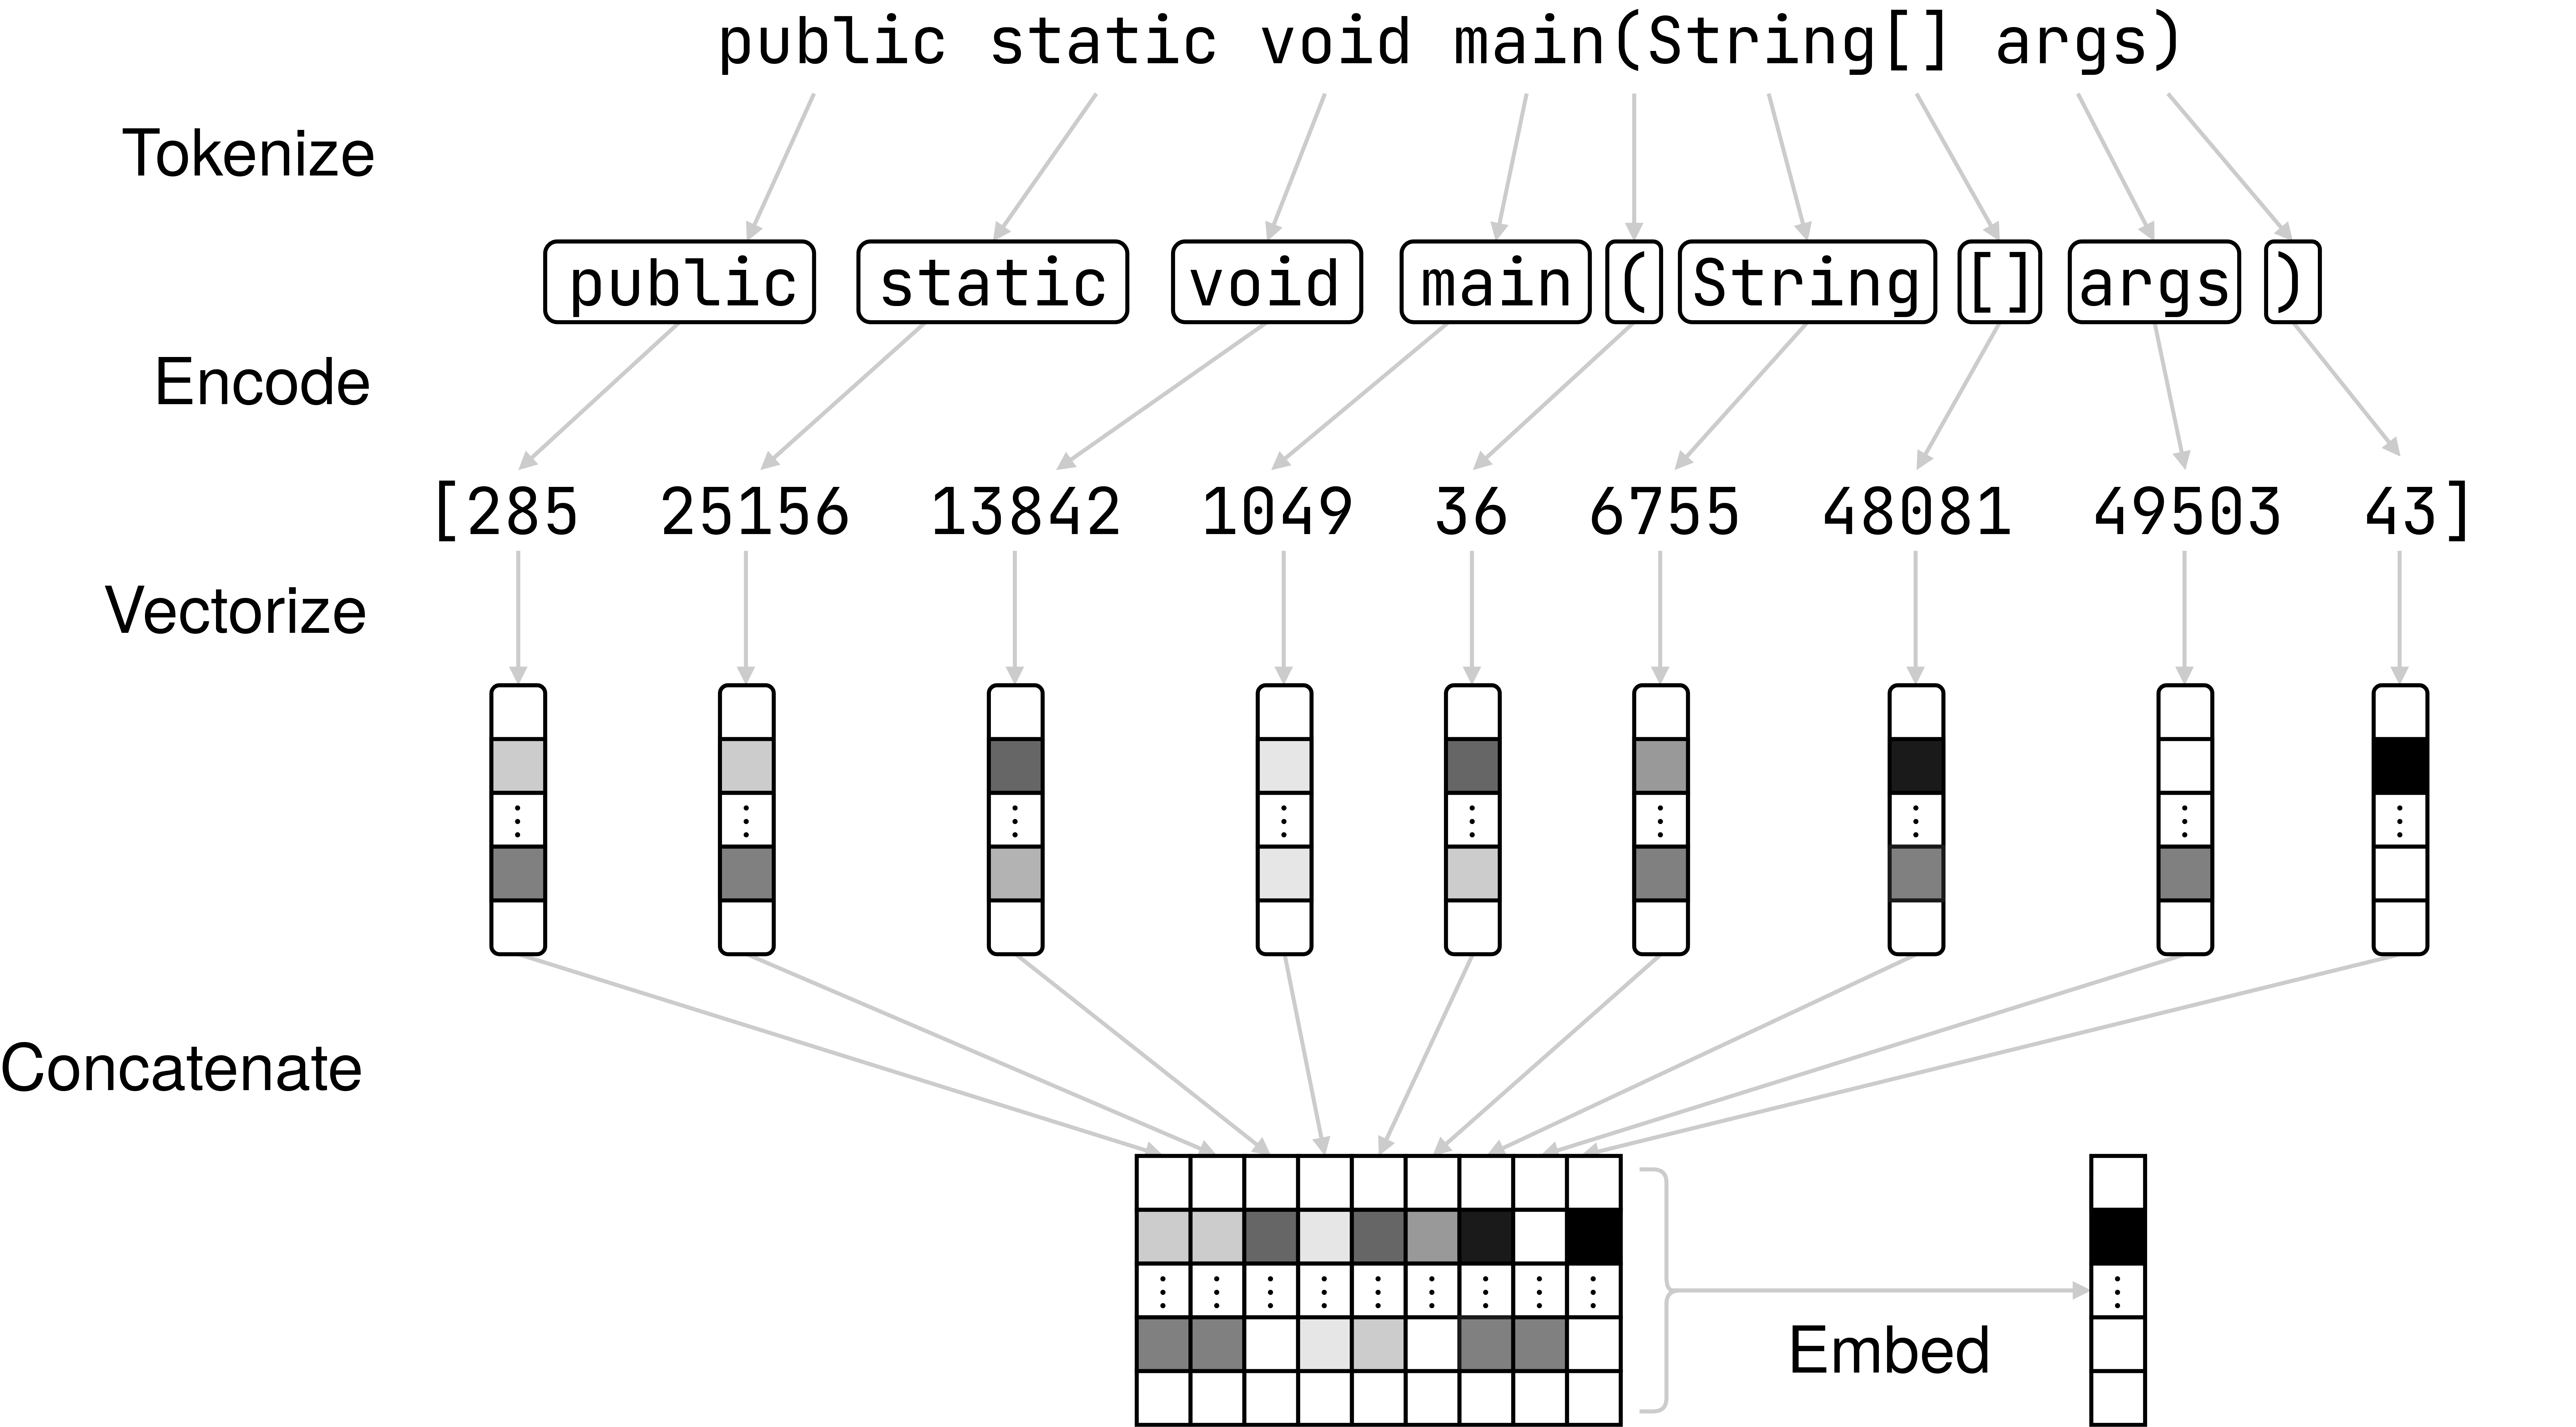
\includegraphics[width=0.40\textwidth]{figs/bert_embedding}
    \caption{CodeBERT takes a unicode sequence and emits a vector sequence, which we accumulate into a single vector.}
    \label{fig:bert}
  \end{figure}

  We evaluate each model under the following four SCTs:

  \begin{enumerate}
    \item The \lstinline|renameTokens| SCT substitutes each CamelCase subword in the most frequent user-defined token with a uniformly-sampled lemma from the WordNet hypernym graph up to three hops away, representing an alternately-chosen [e.g., variable or function] name.
    \item The \lstinline|permuteArgument| SCT performs a Fisher-Yates shuffle on the arguments of a non-JDK function of dyadic or higher-arity, representing an alternate parameter order of a user-defined function.
    \item The \lstinline|swapMultilineNo| SCT swaps adjacent lines of equal scope and indentation which share no tokens in common. Although this may change the semantics of effectful code, in the ideal case, this represents an alternate topological sort on the dataflow graph.
    \item The \lstinline|addExtraLogging| SCT adds intermittent print statements in linear sequences of code, with a single argument synthesized by the code completion model for added variation. More generally, this can be any superfluous statement which does not change the runtime semantics.
  \end{enumerate}

  Idempotent SCTs (i.e., for which the snippet remains unchanged after transformation) are discarded.

  Strictly speaking, we cannot rule out the possibility that any of the aforementioned SCTs produce semantic variants due to the inherent complexity of source code analysis, however we have manually validated their admissibility. A more principled macro system would help to alleviate these concerns, however a framework for safely rewriting isolated Java code snippets is, to the best of our knowledge, presently unavailable.

  To evaluate the effect size of each transformation, we uniformly sample and mask ten tokens from both the original and transformed code snippet, measure the top-1 masked token completion accuracy on the original and transformed code snippet, record the relative difference in accuracy before and after transformation, and finally report the mean and variance for each code complexity bucket.

  \begin{equation}
    E=mc^2
  \end{equation}

  In the following section we report our results for each model, SCT and complexity.

  \pagebreak\section{Results}\label{sec:results}

  We evaluate three state-of-the-art pretrained models on two downstream tasks: code completion and document synthesis. While the sample sizes vary, we provide the same wall clock time (180 minutes) and hardware resources (NVIDIA Tesla V100) to each model. The number of code snippets they can evaluate in the allotted time may vary depending on the architecture, but in each case, the significant figures have mostly converged by this time. Complexity is measured using the procedure described in \S~\ref{sec:slicing}.

  {\center

  CodeBERT
    \begin{table}[H]
      \tiny
      \begin{tabular}{l|cccc}
        Complexity          & \lstinline|renameTokens|        & \lstinline|swapMultilineNo|     & \lstinline|permuteArgument|     & \lstinline|addExtraLogging|     \\\hline\\
        10-20               & -0.13 ± 0.094 (42)  & 0.040 ± 0.329 (156) & 0.208 ± 0.348 (359) & 0.033 ± 0.082 (15)  \\
        20-30               & -0.26 ± 0.189 (112) & 0.137 ± 0.299 (312) & 0.116 ± 0.338 (542) & -0.01 ± 0.202 (82)  \\
        30-40               & -0.29 ± 0.224 (62)  & 0.098 ± 0.264 (163) & 0.185 ± 0.335 (329) & 0.081 ± 0.109 (73)  \\
        40-50               & -0.27 ± 0.222 (74)  & 0.142 ± 0.373 (138) & 0.092 ± 0.357 (232) & 0.043 ± 0.208 (82)  \\
        50-60               & -0.09 ± 0.295 (66)  & 0.041 ± 0.282 (130) & 0.120 ± 0.267 (335) & 0.014 ± 0.181 (136) \\
        60-70               & -0.21 ± 0.244 (60)  & 0.020 ± 0.280 (108) & 0.161 ± 0.252 (179) & -0.02 ± 0.211 (98)  \\
        70-80               & -0.11 ± 0.384 (24)  & 0.071 ± 0.343 (55)  & 0.081 ± 0.376 (79)  & -0.03 ± 0.356 (73)  \\
        80-90               & -0.12 ± 0.325 (42)  & 0.080 ± 0.363 (70)  & 0.035 ± 0.429 (97)  & -0.04 ± 0.350 (75)  \\
        90-100              & -0.04 ± 0.307 (37)  & 0.214 ± 0.291 (52)  & 0.218 ± 0.293 (70)  & 0.075 ± 0.226 (69)  \\
        100-110             & -0.07 ± 0.489 (23)  & 0.149 ± 0.345 (29)  & 0.037 ± 0.427 (44)  & 0.140 ± 0.467 (41)  \\
        110-120             & 0.092 ± 0.335 (18)  & -0.01 ± 0.473 (33)  & -0.04 ± 0.499 (43)  & -0.11 ± 0.236 (32)  \\
        120-130             & 0.076 ± 0.276 (15)  & 0.141 ± 0.235 (13)  & 0.150 ± 0.352 (21)  & 0.111 ± 0.355 (22)  \\
        130-140             & 0.129 ± 0.207 (12)  & 0.178 ± 0.340 (21)  & 0.123 ± 0.349 (27)  & 0.033 ± 0.488 (27)  \\
        140-150             & -0.14 ± 0.387 (9)   & 0.178 ± 0.414 (14)  & 0.107 ± 0.457 (17)  & 0.126 ± 0.542 (19)  \\
      \end{tabular}
    \end{table}


    GraphCodeBERT
    \begin{table}[H]
      \tiny
      \begin{tabular}{l|cccc}
        Complexity          & \lstinline|renameTokens|        & \lstinline|swapMultilineNo|     & \lstinline|permuteArgument|     & \lstinline|addExtraLogging|     \\\hline\\
        10-20               & -0.31 ± 0.204 (21)  & 0.201 ± 0.384 (114) & 0.137 ± 0.374 (276) & 0.166 ± 0.055 (6)   \\
        20-30               & -0.18 ± 0.155 (93)  & 0.130 ± 0.317 (247) & 0.034 ± 0.323 (438) & -0.03 ± 0.209 (71)  \\
        30-40               & -0.19 ± 0.233 (48)  & 0.174 ± 0.209 (149) & 0.198 ± 0.340 (288) & -0.04 ± 0.108 (64)  \\
        40-50               & -0.22 ± 0.256 (61)  & 0.093 ± 0.346 (94)  & 0.078 ± 0.346 (181) & -0.08 ± 0.282 (63)  \\
        50-60               & -0.26 ± 0.228 (59)  & 0.064 ± 0.259 (139) & 0.099 ± 0.280 (323) & -0.06 ± 0.185 (135) \\
        60-70               & -0.21 ± 0.207 (45)  & 0.058 ± 0.251 (85)  & 0.122 ± 0.249 (170) & -0.00 ± 0.224 (82)  \\
        70-80               & -0.39 ± 0.319 (17)  & 0.126 ± 0.417 (46)  & 0.072 ± 0.335 (69)  & -0.11 ± 0.315 (63)  \\
        80-90               & -0.00 ± 0.339 (37)  & -0.00 ± 0.294 (64)  & 0.056 ± 0.340 (85)  & -0.01 ± 0.295 (69)  \\
        90-100              & -0.13 ± 0.291 (29)  & 0.209 ± 0.386 (49)  & 0.035 ± 0.342 (67)  & 0.011 ± 0.254 (61)  \\
        100-110             & -0.18 ± 0.289 (17)  & 0.175 ± 0.377 (31)  & 0.005 ± 0.328 (39)  & 0.074 ± 0.381 (34)  \\
        110-120             & -0.01 ± 0.304 (14)  & 0.130 ± 0.454 (29)  & 0.288 ± 0.469 (34)  & -0.01 ± 0.281 (28)  \\
        120-130             & 0.022 ± 0.505 (10)  & -0.09 ± 0.408 (13)  & -0.13 ± 0.403 (19)  & -0.01 ± 0.367 (20)  \\
        130-140             & 0.033 ± 0.331 (11)  & 0.120 ± 0.406 (20)  & 0.032 ± 0.401 (22)  & 0.005 ± 0.530 (24)  \\
        140-150             & 0.583 ± 0.195 (7)   & -0.04 ± 0.361 (14)  & 0.274 ± 0.290 (17)  & 0.062 ± 0.315 (18)  \\
      \end{tabular}
    \end{table}

    RoBERTa
    \begin{table}[H]
      \tiny
      \begin{tabular}{l|cccc}
        Complexity          & \lstinline|renameTokens|        & \lstinline|swapMultilineNo|     & \lstinline|permuteArgument|     & \lstinline|addExtraLogging|     \\\hline\\
        10-20               & -0.42 ± 0.175 (122) & 0.296 ± 0.406 (277) & 0.387 ± 0.349 (704) & 0.0 ± 0.0 (12)      \\
        20-30               & -0.33 ± 0.172 (168) & 0.258 ± 0.338 (460) & 0.302 ± 0.288 (838) & -0.04 ± 0.145 (101) \\
        30-40               & -0.23 ± 0.188 (107) & 0.084 ± 0.261 (313) & 0.224 ± 0.311 (604) & 0.031 ± 0.172 (142) \\
        40-50               & -0.05 ± 0.237 (118) & 0.183 ± 0.291 (249) & 0.254 ± 0.268 (412) & -3.07 ± 0.098 (155) \\
        50-60               & -0.06 ± 0.239 (108) & 0.085 ± 0.253 (259) & 0.246 ± 0.242 (510) & -0.00 ± 0.138 (203) \\
        60-70               & -0.03 ± 0.196 (80)  & -4.31 ± 0.282 (171) & 0.174 ± 0.273 (291) & -0.02 ± 0.240 (144) \\
        70-80               & 0.124 ± 0.409 (35)  & 0.062 ± 0.253 (97)  & 0.174 ± 0.338 (132) & -0.01 ± 0.235 (107) \\
        80-90               & -0.06 ± 0.394 (43)  & 0.053 ± 0.350 (94)  & 0.225 ± 0.359 (132) & -0.00 ± 0.296 (103) \\
        90-100              & 0.118 ± 0.341 (47)  & 0.064 ± 0.347 (77)  & 0.294 ± 0.339 (95)  & 0.124 ± 0.309 (88)  \\
        100-110             & -0.11 ± 0.454 (32)  & -0.00 ± 0.475 (68)  & -0.00 ± 0.497 (81)  & -0.10 ± 0.411 (59)  \\
        110-120             & -0.16 ± 0.393 (32)  & 0.008 ± 0.498 (57)  & 0.199 ± 0.521 (63)  & -0.02 ± 0.527 (52)  \\
        120-130             & 0.132 ± 0.249 (20)  & 0.155 ± 0.591 (31)  & 0.291 ± 0.378 (41)  & 0.030 ± 0.496 (39)  \\
        130-140             & 0.111 ± 0.328 (18)  & 0.027 ± 0.519 (39)  & 0.256 ± 0.463 (46)  & 7.575 ± 0.494 (44)  \\
        140-150             & 0.265 ± 0.370 (23)  & 0.109 ± 0.575 (32)  & 0.357 ± 0.311 (33)  & 0.201 ± 0.500 (33)  \\
        150-160             & -0.04 ± 0.602 (12)  & 0.214 ± 0.407 (21)  & 0.064 ± 0.487 (26)  & 0.125 ± 0.512 (24)  \\
      \end{tabular}
    \end{table}
  }
  
  As we can see, RoBERTa is considerably more sensitive to cosmetic variance than CodeBERT and GraphCodeBERT. In all cases, the  \lstinline|swapMultilineNo| and \lstinline|permuteArgument| SCTs exhibit a more detrimental effect than the \lstinline|renameTokens| or \lstinline|addExtraLogging| SCTs. Counterintuitively, it appears that token renaming tends to improve completion accuracy across all models on average.


  \begin{tikzpicture}
    \begin{axis}[
      ymin=0, ymax=55,
      minor y tick num = 3,
      symbolic x coords = {CodeBERT, GraphCodeBERT, RoBERTa},
      area style,
    ]
      \addplot+[ybar interval,mark=no] plot coordinates { (LaTeX, 5) (Tools, 35) (Distributions, 50)} ;
    \end{axis}
  \end{tikzpicture}
  

  Documentation Generation
    {
    \renewcommand{\arraystretch}{1.5}
    \begin{table}[H]
      \footnotesize
      \begin{tabular}{l|ccc}
        Model & Low Complexity & Medium Complexity & High Complexity \\
        \hline
        \href{https://huggingface.co/microsoft/CodeGPT-small-java}{\textsc{CodeGPT}}~\citep{lu2021codexglue} & X & X & X \\
        \href{https://huggingface.co/microsoft/graphcodebert-base}{\textsc{GraphCodeBERT}}~\citep{guo2021graphcodebert} & Rougescore & Rougescore & Rougescore \\
        \href{https://huggingface.co/huggingface/CodeBERTa-small-v1a}{\textsc{CodeBERT-small}}~\citep{feng2020codebert} & Rougescore & Rougescore & Rougescore \\
        \href{https://huggingface.co/dbernsohn/roberta-java}{\textsc{RoBERTa-Java}}~\citep{liu2019roberta} & Rougescore & Rougescore & Rougescore \\
        \href{https://copilot.github.com/}{\textsc{Copilot}}\citep{chen2021evaluating} & Rougescore & Rougescore & Rougescore \\

      \end{tabular}
      \caption{\label{tab:doc_synthesis} Experiments table for comparing pretrained LM embeddings on source code snippets. IRA: Iterrater agreement. QDL: query description length, P/R: Precision/recall}
    \end{table}
  }

    {
    \renewcommand{\arraystretch}{1.5}
    \begin{table}[H]
      \footnotesize
      \begin{tabular}{l|ccc}
        Model & Low Complexity & Medium Complexity & High Complexity \\
        \hline
        \href{https://huggingface.co/microsoft/CodeGPT-small-java}{\textsc{CodeGPT}}~\citep{lu2021codexglue} & X & X & X \\
        \href{https://huggingface.co/microsoft/graphcodebert-base}{\textsc{GraphCodeBERT}}~\citep{guo2021graphcodebert} & P/R & P/R & P/R \\
        \href{https://huggingface.co/huggingface/CodeBERTa-small-v1a}{\textsc{CodeBERT-small}}~\citep{feng2020codebert} & P/R & P/R & P/R \\
        \href{https://huggingface.co/dbernsohn/roberta-java}{\textsc{RoBERTa-Java}}~\citep{liu2019roberta} & P/R & P/R & P/R \\
        \href{https://copilot.github.com/}{\textsc{Copilot}}\citep{chen2021evaluating} & P/R & P/R & P/R \\

      \end{tabular}
      \caption{\label{tab:code_completion} Experiments table for comparing pretrained LM embeddings on source code snippets. IRA: Iterrater agreement. QDL: query description length, P/R: Precision/recall}
    \end{table}
  }

  \section{Discussion}


  We can also reproduce the relative rankings of the models as reported in relevant literature: RoBERTa $<<$ CodeBERT $<$ GraphCodeBERT.

  We observe a clear trend over method complexity: SCTs in low complexity code have a larger effect than similar transformations in high-complexity code. We hypothesize this trend can be explained by the fact that rewriting can have comparatively large effect when the surrounding code snippet is tiny and therefor contains less contextual information.

  If we examine the source code snippets, we notice that renaming can have a significant effect on document synthesis. Examining the synthesized documents, we can see that the model frequently copies tokens from the source code, so renaming can degrade document quality. Similarly swapping multiline statements also reduces document quality.\ldots

  \pagebreak
  \section{Conclusion}\label{sec:conclusion}

  The work described herein is primarily an empirical study, but also represents a framework and a set of methodological practices which may be used to evaluate future code-based neural language models, offering several advantages from a software engineering standpoint. Due to its functional implementation, it is efficient, parallelizable and highly modular. Further details about the architecture and its benefits can be found in \S~\ref{sec:architecture}.

  Despite its simplicity, the Regex-based SCT approach has some shortcomings. While regular expressions are simple to implement and support rudimentary transformations, they are a crude way to manipulate source code. In order to generate semantically valid transformations, one must really use full-fledged term rewriting system, such as higher-order abstract syntax or some kind of parser-combinator. Several options were evaluated, including OpenRewrite, TXL, Refal et al., but their features and complexity were ultimately found wanting.

  We have identified four rewriting categories, corresponding to possible types of source code transformations:

  \begin{enumerate}
    \item Syntactic - can the LM detect syntactically invalid PTs? (e.g. syntax corruption, imbalanced parenthesis)
    \item Structural - can the LM detect syntactically valid, but semantically unsound PTs? (e.g. use before declaration, permuted argument order)
    \item Semantic - can the LM detect semantically valid, but semantically altered PTs? (e.g. constant modification, operator substitution and order of operations)
    \item Cosmetic - can the LM detect syntactically and semantically equivalent PTs? (e.g. variable renaming, documentation)
  \end{enumerate}

  The present work falls into the latter-most category, however other types of SCTs may be considered in future work. Furthermore, while we currently only use mutlimask accuracy at top-1 and ROUGE-synonym score, we hope to compare various other metrics such as mean average precision, MRR, NDCG, interrater agreement and others in the future.

  Neural language models hold much promise for improved code completion, however complacency can lead to increased reviewer burden or more serious technical debt if widely adopted. While trade secrecy may prevent third-party inspection of pretrained models, users would still like some assurance of the model's robustness to naturally-occurring variance. Our work helps to address this by generating plausible cosmetic variants and measuring end-to-end robustness of the neural language model.
  \pagebreak\bibliography{main}
  \bibliographystyle{plain}
  \pagebreak
  \appendix

  \section{Slicing procedure}\label{sec:slicing}

  We describe below a simple heuristic for extracting method slices in well-formed source code using a Dyck counter.~\footnote{\url{https://en.wikipedia.org/wiki/Dyck\_language}} A common coding convention is to prefix functions with a keyword, followed by a group of balanced brackets and one or more blank lines. While imperfect, we observe this pattern can be used to slice methods in a variety of languages in practice. A Kotlin implementation is given below, which will output the following source code when run on itself:

  \vspace{11pt}

  \begin{lstlisting}[basicstyle=\scriptsize\ttfamily, language=kotlin,label={lst:example4}]
fun String.sliceIntoMethods(kwds: Set<String> = setOf("fun ")) =
  lines().fold(-1 to List<String>(0)) { (dyckCtr, methods), ln ->
    if (dyckCtr < 0 && kwds.any { it in ln }) {
      ln.countBalancedBrackets() to (methods + ln)
    } else if (dyckCtr == 0) {
      if (ln.isBlank()) -1 to methods else 0 to methods.put(ln)
    } else if (dyckCtr > 0) {
      dyckCtr + ln.countBalancedBrackets() to methods.put(ln)
    } else -1 to methods
  }.second

fun List<String>.put(s: String) = dropLast(1) + (last() + "\n$s")

fun String.countBalancedBrackets() = fold(0) { sum, char ->
  val (lbs, rbs) = setOf('(', '{', '[') to setOf(')', '}', ']')
  if (char in lbs) sum + 1 else if (char in rbs) sum - 1 else sum
}

fun main(args: Array<String>) =
  println(args[0].sliceIntoMethods().joinToString("\n\n"))
  \end{lstlisting}

  Using this approach, we can approximate the bracket complexity for each code snippet and slice methods horizontally. More elaborate dataflow-based slicing procedures require parsing.

  \section{Architectural details}\label{sec:architecture}

  Our experimental architecture is to our knowledge, unique, and merits some discussion. The entire pipeline from data mining to preprocessing, evaluation and table generation is implemented as a pure functional program in the point-free style, enabling straightforward parallelization.

  We can view the tables in this paper as 2D-slices of a rank-n tensor representing an n-dimensional hyperdistribution formed by the Cartesian product of all variables under investigation (e.g. code complexity, metric, task, model). During evaluation, we sample the independent variables uniformly to ensure its entries are evenly populated. Results are continuously delivered to the user, who may preview 2D marginals for any pair and watch the error bounds grow tighter as additional samples are drawn.

  This kind of feature is useful when running on preemptible infrastructure and can be massively parallelized to increase the experiment's statistical power or explore larger subspaces of the experimental design space.

  \pagebreak\section{Analysis of internal structure}\label{sec:probe_internals}

  Our preliminary results compare distance metrics (Fig.~\ref{fig:lev_vs_euclid}), explore embedding quality (Fig.~\ref{fig:embedding}) and visualize the synthetic knowledge graphs (Fig.~\ref{fig:graphs}).

  In the figure below, we compute the distance between pairs of random code snippets in CodeBERT latent space and find a positive correlation with various string distance metrics.

  \begin{figure}[H]
    \centering
    \resizebox{0.45\textwidth}{!}{%
      \begin{tikzpicture}
        \begin{axis}[width=0.29\textwidth, height=0.3\textwidth, ymax=7, xlabel=Levenshtein, ylabel=Euclidean]
          \addplot table [mark=none,x=strdist, y=embdist, variable=var, col sep=comma] {data/levenshtein.csv};

          \addplot [smooth, name path=upper,draw=none] table[x=strdist, y=embdist,variable=var, y expr=\thisrow{embdist}+\thisrow{var}, col sep=comma] {data/levenshtein.csv};
          \addplot [smooth, name path=lower,draw=none] table[x=strdist, y=embdist,variable=var, y expr=\thisrow{embdist}-\thisrow{var}, col sep=comma] {data/levenshtein.csv};
          \addplot [fill=red!10] fill between[of=upper and lower];
        \end{axis}
      \end{tikzpicture}
      \begin{tikzpicture}
        \begin{axis}[width=0.29\textwidth, height=0.3\textwidth, ymax=7, xlabel=Damerau]
          \addplot table [mark=none,x=strdist, y=embdist, variable=var, col sep=comma] {data/damerau.csv};

          \addplot [smooth, name path=upper,draw=none] table[x=strdist, y=embdist,variable=var, y expr=\thisrow{embdist}+\thisrow{var}, col sep=comma] {data/damerau.csv};
          \addplot [smooth, name path=lower,draw=none] table[x=strdist, y=embdist,variable=var, y expr=\thisrow{embdist}-\thisrow{var}, col sep=comma] {data/damerau.csv};
          \addplot [fill=red!10] fill between[of=upper and lower];
        \end{axis}
      \end{tikzpicture}
      \begin{tikzpicture}
        \begin{axis}[width=0.29\textwidth, height=0.3\textwidth, ymax=7, xlabel=MetricLCS]
          \addplot table [mark=none,x=strdist, y=embdist, variable=var, col sep=comma] {data/metriclcs.csv};

          \addplot [smooth, name path=upper,draw=none] table[x=strdist, y=embdist,variable=var, y expr=\thisrow{embdist}+\thisrow{var}, col sep=comma] {data/metriclcs.csv};
          \addplot [smooth, name path=lower,draw=none] table[x=strdist, y=embdist,variable=var, y expr=\thisrow{embdist}-\thisrow{var}, col sep=comma] {data/metriclcs.csv};
          \addplot [fill=red!10] fill between[of=upper and lower];
        \end{axis}
      \end{tikzpicture}
      \begin{tikzpicture}
        \begin{axis}[width=0.29\textwidth, height=0.3\textwidth, ymax=7, xlabel=Jaccard]
          \addplot table [mark=none,x=strdist, y=embdist, variable=var, col sep=comma] {data/jaccard.csv};

          \addplot [smooth, name path=upper,draw=none] table[x=strdist, y=embdist,variable=var, y expr=\thisrow{embdist}+\thisrow{var}, col sep=comma] {data/jaccard.csv};
          \addplot [smooth, name path=lower,draw=none] table[x=strdist, y=embdist,variable=var, y expr=\thisrow{embdist}-\thisrow{var}, col sep=comma] {data/jaccard.csv};
          \addplot [fill=red!10] fill between[of=upper and lower];
        \end{axis}
      \end{tikzpicture}
    }
    \caption{CodeBERT latent space vs. string edit distance.}
    \label{fig:lev_vs_euclid}
  \end{figure}

  \begin{figure}[H]
    \centering
    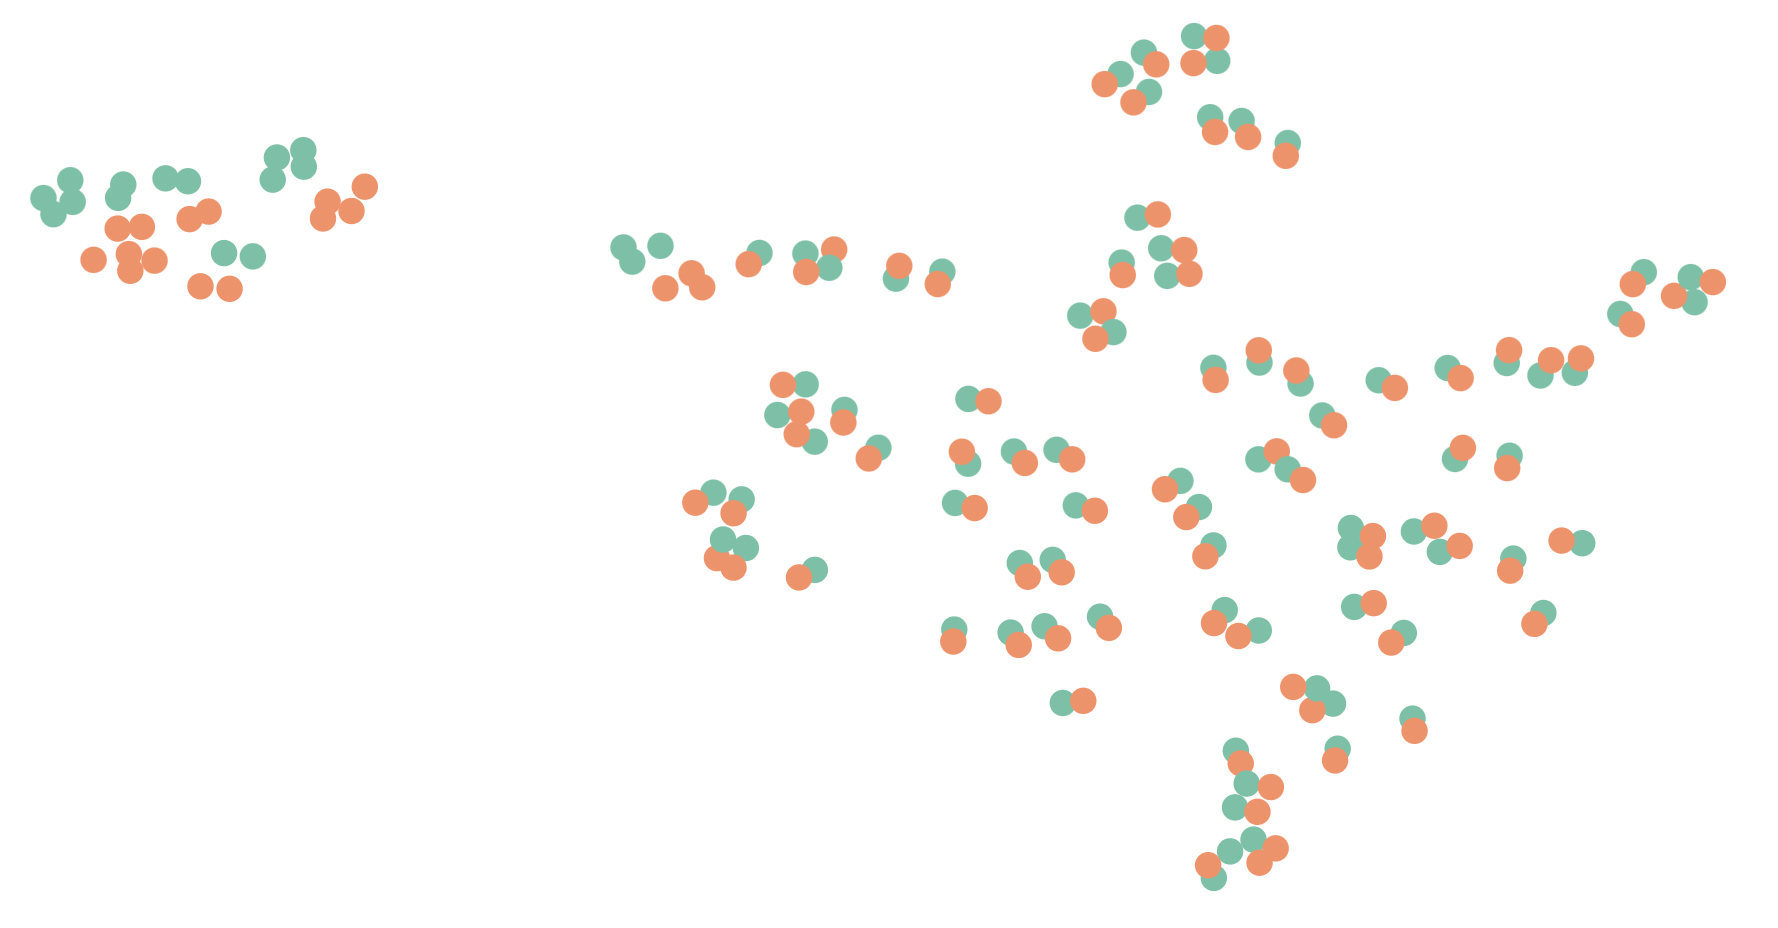
\includegraphics[width=0.4\textwidth]{figs/rename_tokens}
    \caption{TSNE-embedded code snippets before (green) and after (orange) synonym renaming was applied.}
    \label{fig:embedding}
  \end{figure}

  We fetch a dataset of Java and Kotlin repositories sampled repositories on GitHub, containing a mixture of filetypes representing source code and natural language artifacts.
%
  From each repository, we index all substrings of every line in every file using a variable height radix tree producing a multimap of $\texttt{kwdIndex: String -> List<Location<F, O>>}$ of $\texttt{String}$  queries to file-offset pairs. We also encode CodeBERT~\citep{feng2020codebert} sequence embeddings to substrings $\texttt{knnIndex: Vector -> Location<F, O>}$ using a Hierarchial Navigavble Small World Graph~\citep{malkov2018efficient} (HNSWG).


  \begin{figure}[H]
    \centering
    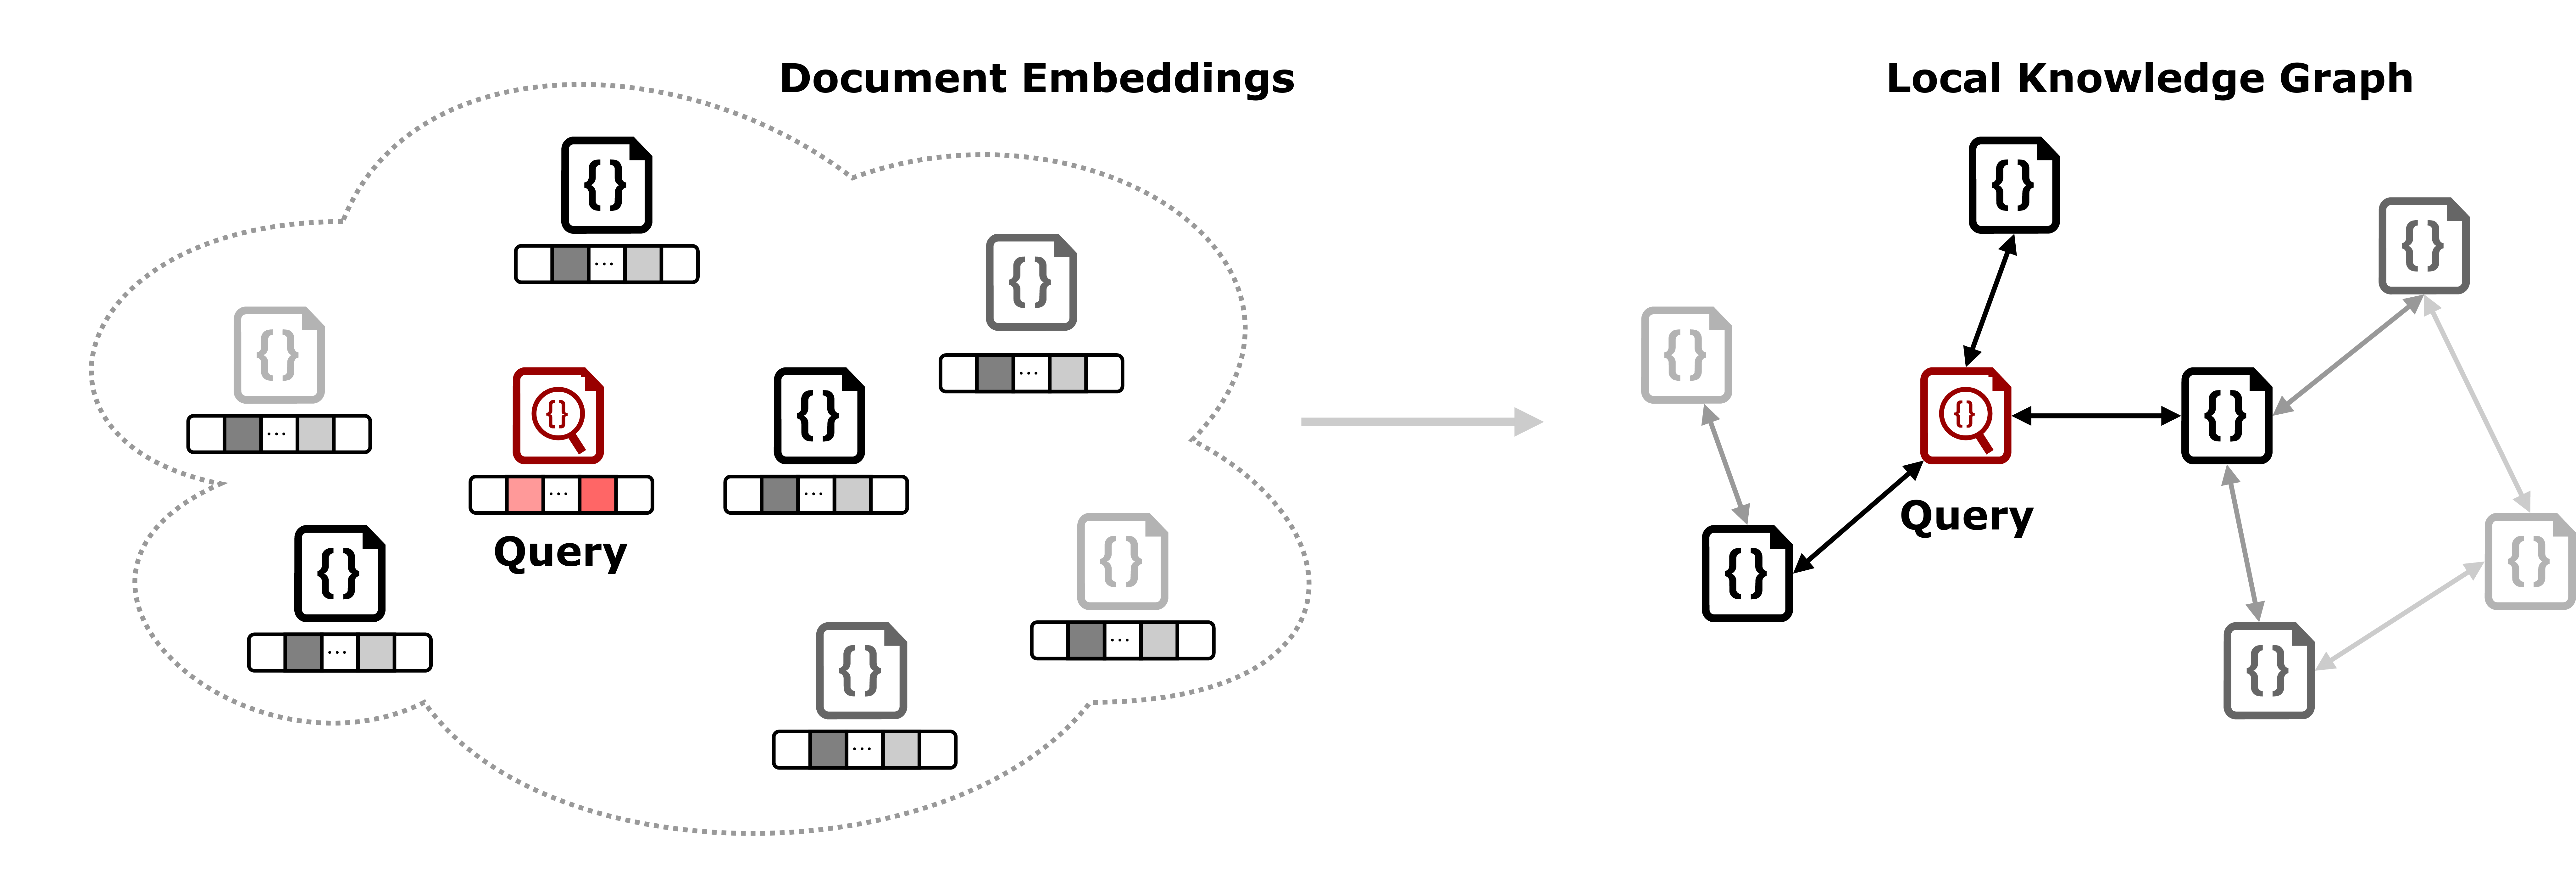
\includegraphics[width=0.4\textwidth]{figs/latent_kg}
    \caption{To compute our query neighborhood, we traverse the HNSWG up to max depth $d$, i.e. $d=1$ fetches the neighbors, $d=2$ fetches the neighbors-of-neighbors, and $d=3$ fetches the neighbors-of-neighbors-of-neighbors.}
    \label{fig:de2kg}
  \end{figure}

  \begin{figure}[H]
    \centering
    \resizebox{.1\textwidth}{!}{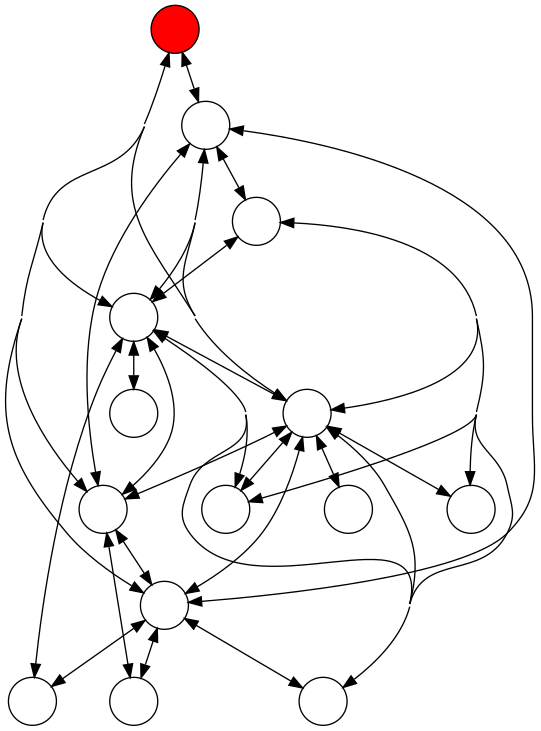
\includegraphics{../data/query4}}
    \resizebox{.1\textwidth}{!}{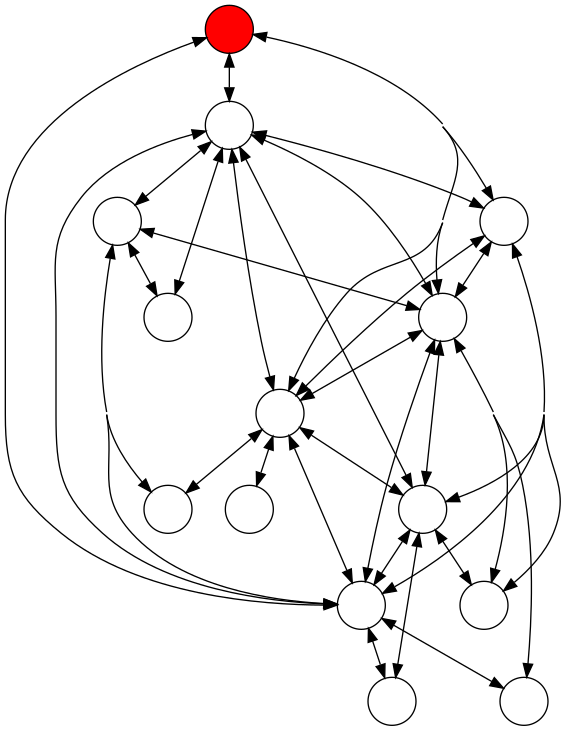
\includegraphics{../data/query5}}
    \resizebox{.1\textwidth}{!}{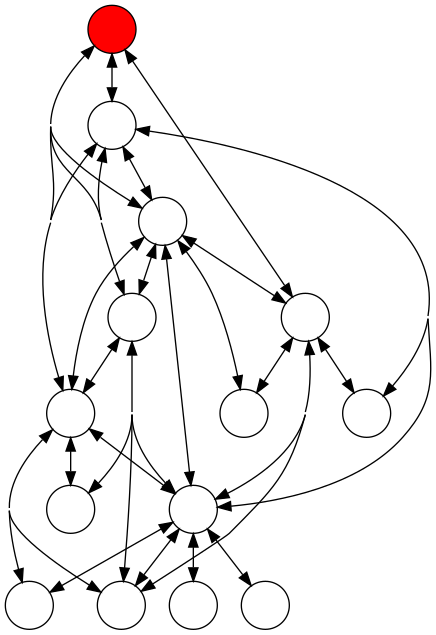
\includegraphics{../data/query6}}
    \resizebox{.1\textwidth}{!}{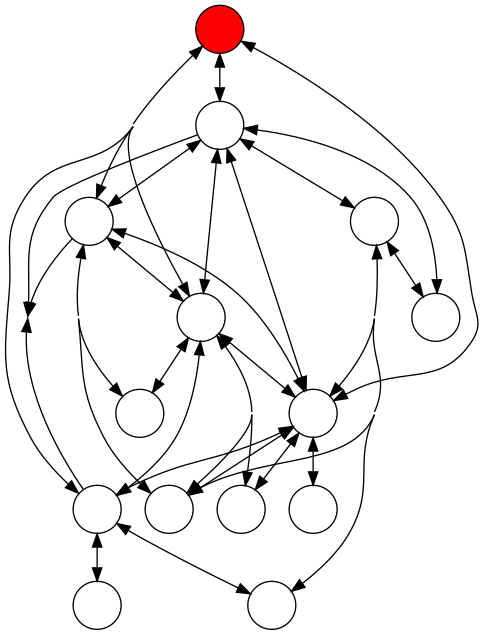
\includegraphics{../data/query7}}
    \resizebox{.1\textwidth}{!}{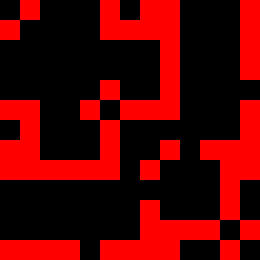
\includegraphics{../data/context4}}
    \resizebox{.1\textwidth}{!}{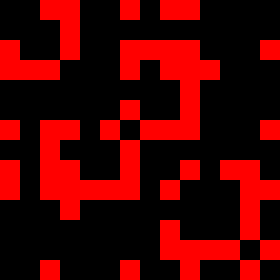
\includegraphics{../data/context5}}
    \resizebox{.1\textwidth}{!}{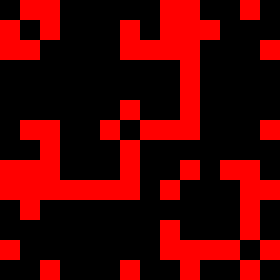
\includegraphics{../data/context6}}
    \resizebox{.1\textwidth}{!}{
\includegraphics{../data/context7}}
    \caption{Virtual knowledge graph constructed by searching Euclidean nearest-neighbors in latent space. Edges represent the k-nearest neighbors, up to depth-n (i.e., k=5, n=3).}
    \label{fig:graphs}
  \end{figure}


\end{document}
\endinput